\externaldocument{modelling}

\section{Method}

%correct systematic variation table

This work will investigate how the free parameters of the model given by the equations~\ref{eq:6} -~\ref{eq:10} will affect the spatial temporal progress of the numerical simulation. For the numerical simulation we will use the weak form given with equations~\ref{eq:11} -~\ref{eq:13} and solve it using HiFlow. To study the results of the numerical simulation ParaView is used, producing informative plots to compare the evolution of the simulation in time. For this we rely on the tool Plot Over Line to give radially symmetrical reulsts of the three variables of tumour and extracellular matrix density and matrix-degrading enzymes, an example for this can be seen in figure~\ref{fig:Initial_Value_Distribution} showing the initial conditions. In figure~\ref{fig:PlotOverLine} you can see the configuraion for the Plot Over Line tool, since we are consider the experiments on the unit squre in 2D dimensional case, the line starts at $x=0.5, y=0.5$ and ends at $x=0.5, y=1$.\newline
\begin{figure}[h]
    \centering
    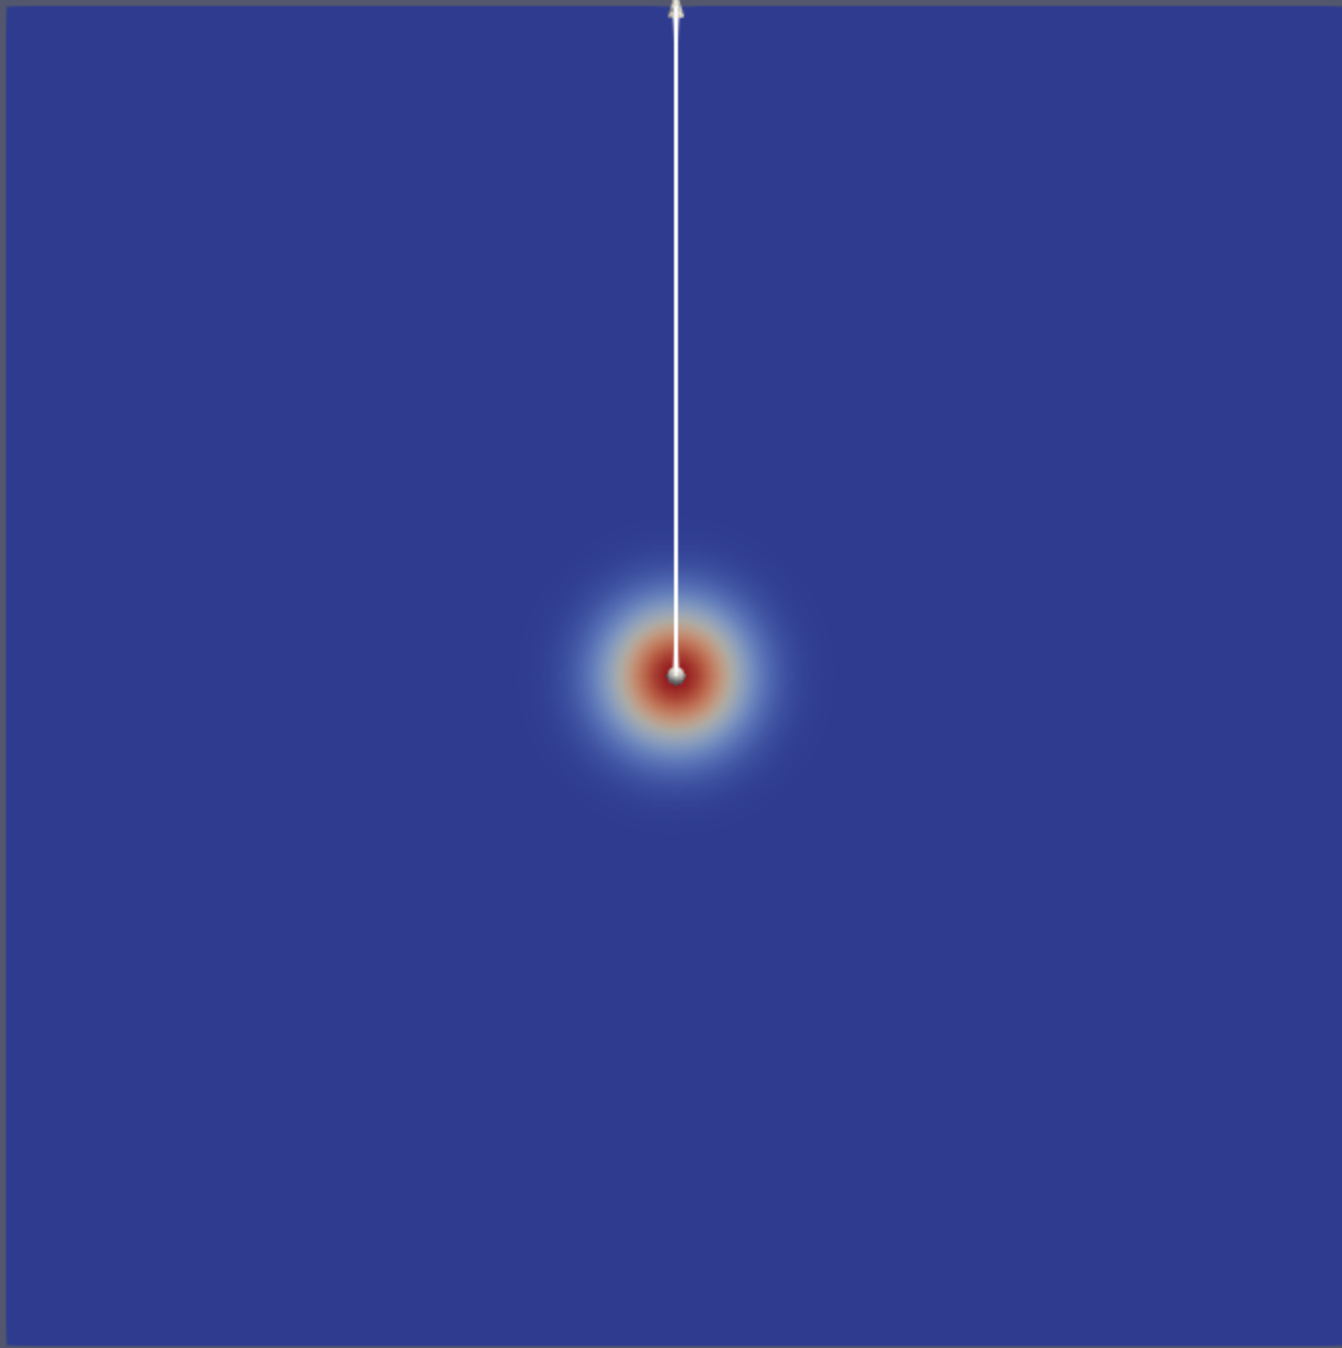
\includegraphics[width=0.3\textwidth]{resources/images/plot_over_line_tool.png}
    \caption{Plot Over Line Tool Configuration}
    \label{fig:PlotOverLine}
\end{figure}
For the three dimensional experiments a different tool was used ....$\textcolor{red}{explain 3D experients methodology}$
All experiments that consider the ECM to be homogenous start with the same initial values as seen in figure~\ref{fig:Initial_Value_Distribution}. Experiments observing the effects of a heterogenous ECM use different initial values, like seen in $\textcolor{red}{initial values heterogenous ECM}$\newline 
This work starts with \textcolor{red}{trying to replicate/replicating} numerical simulations done by other papers. Since there were only 1D simulations done previously, the model will be adjusted in such a way, that the Plot Over Line graphs mimick the plots given by the previous experiments. This will serve two purposes, first and minor it will verify a correct implemntation of the model and second this will give us a starting point by which we can vary the parameters, investigating the phenomena this model exhibits. \newline 
We will start with exmaining 2D experiments with homogenous ECMs, using our model with the parameters $mu_1$ and $mu_2$ both set to zero, considering a case with no proliferation, after this we will introduce proliferation, varying also $mu_1$ and $mu_2$. The same will be done for the 3D cases, also at first neglecting proliferation to apply it in a later stage. Our focus here lies on investigating the effects of the parameters, but also on how the dimension changes results, with fixed free parameters. At last we will have a brief outlook on how a heterogenous ECM influences our results\newline
The results of the above experiments will be summarized and discussed in the Conclusion and Discussion part, pointing out the important characteristics of the simulations and disucssing the sensitivity of each of the parameters and the influence of the dimension. At this point we will have an outlook on how to extend the model with more continuous and or discrete adaptations. \newline \newline

Looking at the parameter estimates from \cite{anderson_mathematical_2000} to non-dimensionalise the time, we see that with $L \in [0.1cm,1cm]$ and $D\approx 10^{-6}\frac{cm^2}{s}$, $\tau = \frac{L^2}{D}$ gives a relative big temporal range, $\tau_{min} = 1000s = 16.66 min$ and $\tau_{max} = 1000000s = 16666.66min$, which makes it hard, to find the correct time step value to compare our simulation results with the one from \cite{anderson_mathematical_2000} and \cite{Kolev2010}. Another challenge are the diffusion coefficients, since they are dependent on the dimension we are in, we have to find our own estimate as a baseline value. \newline 
For our experiments we will use a set of baseline parameters, which will be evaluated experimentally, and from there vary one parameter at a time to get a overview of their effects and later we will incorporate variation of multiple paramters in accordance with the numerical model. 


\begin{comment}

    For each of the modified free parameters $d_c, \gamma, \eta, d_m, \alpha, \beta, \mu_1, \mu_2$ we are going to take look at values or ranges which were used in previous experiments: 
\begin{itemize}
    \item $d_c = 0.001$
    \item $\gamma \in \{0.001, 0.002, 0.005\}$
    \item $\mu_1 \in \{0.1, 0.5\}$
    \item $\eta \in \{10, 20\}$
    \item $\mu_2 \in \{0.1, 0.5\}$
    \item $d_m \in \{0.001, 0.01\}$
    \item $\alpha \in \{0.1, 10\}$
    \item $\beta \in \{0, 0.07, 0.5\}$
\end{itemize}


\begin{table}[!h]
    \begin{center}
        \label{tab:systematic_analysis}
        \begin{tabular}{||c c c c||} 
            \hline
            Col1 & Col2 & Col2 & Col3 \\ [0.5ex] 
            \hline\hline
            1 & 6 & 87837 & 787 \\ 
            \hline
            2 & 7 & 78 & 5415 \\
            \hline
            3 & 545 & 778 & 7507 \\
            \hline
            4 & 545 & 18744 & 7560 \\
            \hline
            5 & 88 & 788 & 6344 \\ [1ex] 
            \hline
        \end{tabular}
        \caption{Your caption.}
    \end{center}
\end{table}

Looking at the estimates of section 3 we are left with plenty of room to investigate the effects of every single parameter. For this systematic analysis we are going to assume a baseline set of parameters, $(d_c, \gamma, \mu_1, \eta, \mu_2, d_m, \alpha, \beta) = (0.001, 0.005, 0, 10, 0, 0.001,0.1, 0)$ for experiments without proliferation and \newline
$(d_c, \gamma, \mu_1, \eta, \mu_2, d_m, \alpha, \beta) = (0.001, 0.005, 0.3, 10, 0.3, 0.001,0.1, 0.1)$ for experiments with proliferation, where in every experiment one paramter will be changed. Later this will be extended to study a cross-analysis, where more than one parameter is changed at a time. The set of baseline parameters is taken from previous experiments done by Anderson et al.~\cite{anderson_mathematical_2000} and Kolev et al.~\cite{Kolev2010}. The systematic variations will be same for 2D as well as 3D experiments and can be found in talbe~\ref{tab:systematic_analysis}.

\subsection{Software and Implementation}
\subsection{Systematic Parameter Analysis}
\subsubsection{2D}
\subsubsection{3D}
\subsubsection{Non-heterogenous ECM Structure}

This work will investigate how the results of the modified model in the modelling section will be affected be varying free parameters $\lambda, \delta, \mu_1, \mu_2, \mu_3$ as well as how the chosen dimension for a simulation will influence the output.
For this we will start with comparing results first within the same dimension, varying the free parameters. Conducting these experiments we hope that we can see a pattern occuring, which is shared across one dimension. After this we will investigate how the results are changed when we change the dimension but keep the free parameters the same. 


\begin{center}
\begin{tabular}{|| c | c | c | c | c || c | c | c | c | c || c | c | c | c | c ||}
    \hhline{||=|=|=|=|=||=|=|=|=|=||=|=|=|=|=||}
    1D \small & & & & & 2D & & & & & 3D & & & & \\
    \hhline{||=|=|=|=|=||=|=|=|=|=||=|=|=|=|=||}
    $\lambda$ & $\delta$ & $\mu_1$ & $\mu_2$ & $\mu_3$  & $\lambda$ & $\delta$ & $\mu_1$ & $\mu_2$ & $\mu_3$ & $\lambda$ & $\delta$ & $\mu_1$ & $\mu_2$ & $\mu_3$ \\ 
    \hline
    a & b & c & d & e & a & b & c & d & e & a & b & c & d & e \\ \hline 
    a & b & c & d & e & a & b & c & d & e & a & b & c & d & e \\ \hline 
    a & b & c & d & e & a & b & c & d & e & a & b & c & d & e \\ \hline 
    a & b & c & d & e & a & b & c & d & e & a & b & c & d & e \\ \hhline{||=|=|=|=|=||=|=|=|=|=||=|=|=|=|=||} 

\end{tabular}
\end{center}

When comparing the effects of the free parameters on the simulation we need to keep in mind, that some of them are by assupmtion fixed, whilst others are defined within a reasonable range and again others have no restrictions at all, for those we assume the value ranges in the modelling section. At this first stage of the investigation we change only one parameter within each group of experiments, for example we only study how the output changes when $\delta$ changes, we do this with every parameter and compare the results within their dimension. When we are done with that we compare the results with changing dimension whilst keeping every other free parameter equal. \newline
With the core question that if different dimensions yield different results, we hope to find characteristics prevailing in each dimension, but mainly concentrate on the features that arise with the same choice of parameters varying the dimension. We hope to find answers to which changes in outcome emerge and how to explain the different results. \newline
As a last step this work compares the found results with clinical results, from in-vitro results. Why in-vitro, because this models lacks the biological complexity which governs many effects regarding tumor growth in living bodies, which would yield to quite different behaviour.
\end{comment}